\chapter{Technische Grundlagen}
\label{cha:Technische Grundlagen}

Dieses Kapitel gibt einen Überblick über die wichtigsten technischen Konzepte und Methoden, die für das Verständnis moderner Dokumentenverarbeitungssysteme grundlegend sind. Dabei werden sowohl grundlegende Konzepte als auch Metriken zur Messung des Erfolgs bearbeitet. 

\section{Optical Character Recognition (OCR)}
\label{sec:optical-character-recognition-ocr}

\gls{OCR} ist eine Schlüsseltechnologie bei der Verarbeitung von visuellen Dokumenten. Sie erfüllt die Aufgabe, Bilder von gedrucktem oder handgeschriebenem Text in maschinenlesbaren Text umzuwandeln \cite{MoriS.1992HroO}.
Auch wenn \gls{OCR} für Optical Character Recognition steht, erkennen viele der gängigen Systeme in Wahrheit Zeichenblöcke oder ganze Wörter \cite{BorovikovEugene2014Asom}.
Es gibt eine Vielzahl an verschiedenen \gls{OCR} Methoden, von denen einige Segmentierung, also die Zuteilung jedes Pixels zu einer Kategorie, verwenden und andere nicht \cite{BorovikovEugene2014Asom}. Die meisten modernen \gls{OCR}-Systeme bestehen dabei typischerweise aus zwei essenziellen Teilen \cite{BorovikovEugene2014Asom}:

\begin{enumerate}
    \item Feature Extractor: Basierend auf einem Bild eines Elements extrahiert dieser die charakteristischen Merkmale (Deskriptoren) des Elements. Diese abgeleiteten Merkmale dienen als Eingabe für den Classifier.
    \item Classifier: Dieser bestimmt anhand der extrahierten Merkmale das (wahrscheinlichste) bekannte Element. Zusätzlich liefert der Classifier einen Konfidenzwert, der angibt, wie sicher die Erkennung des Elements ist.
\end{enumerate}

Diese grundlegende Struktur bildet die Basis für verschiedene klassische und moderne Methoden der optischen Zeichenerkennung \cite{BorovikovEugene2014Asom}:

\begin{itemize}
\item Template Matching: Vergleicht Eingabezeichen pixelweise mit bekannten Vorlagen und wählt die ähnlichste aus.
\item Strukturelle Klassifikation: Nutzt strukturelle Merkmale wie Striche, Löcher oder Ecken und wendet regelbasierte Systeme an.
\end{itemize}

Dabei ist zu beachten, dass es auch leichte Abweichungen und hybride Varianten von diesen Techniken gibt \cite{BorovikovEugene2014Asom}. Viele moderne \gls{OCR}-Systeme verwenden mathematische Funktionen, die darauf abzielen, eine Metrik der Abweichung von einer Vorlage zu minimieren; Beispiele dafür sind \cite{BorovikovEugene2014Asom}:

\begin{itemize}
    \item Diskriminanzfunktionen: Verwenden Hyperebenen im mehrdimensionalen Merkmalsraum zur Trennung von Zeichenklassen.
    \item Bayes-Klassifikatoren: Minimieren Fehlklassifikationen mittels Wahrscheinlichkeitstheorie.
    \item Künstliche Neuronale Netze (KNN): Lernen komplexe Klassifikationsabbildungen durch Fehlerrückführung und Optimierungstechniken.
\end{itemize}

\subsection{Tesseract OCR}
\label{subsec:tesseract-ocr}
Das für die im Rahmen dieser Bachelorarbeit implementierten Prototypen verwendete \gls{OCR}-System heißt Tesseract \gls{OCR}. Dabei handelt es sich um ein ursprünglich von Hewlett Packard entwickeltes \gls{OCR}-System, welches seit 2005 als Open-Source-Software verfügbar ist \cite{SmithR_2007_AOot}. Tesseract basiert auf \gls{LSTM} neuronalen Netzen, welches über 100 Sprachen und über 35 Schriftsysteme unterstützt \cite{tesseract_ocr_user_manual}. 

\subsubsection{Architektur und Funktionsweise}
\label{subsubsec:architektur-und-funktionsweise}
Tesseract folgt einem traditionellen Pipeline-Ansatz für die Texterkennung, wobei einige Schritte zur Zeit ihrer Entwicklung ungewöhnlich waren \cite{SmithR_2007_AOot}. Der Prozess beginnt mit einer Analyse verbundener Komponenten, bei der die Umrisse der Komponenten gespeichert werden. Diese Methode ermöglicht es Tesseract, sowohl schwarzen Text auf weißem Hintergrund als auch umgekehrt zu erkennen \cite{SmithR_2007_AOot}.

\subsubsection{Zeilenfindung und Basislinienanpassung}
\label{subsubsec:zeilenfindung-und-basislinienanpassung}
Ein wichtiger Aspekt von Tesseract ist der Algorithmus zur Zeilenfindung, der es ermöglicht, schiefe Seiten ohne vorherige Entzerrung zu erkennen. Dies verhindert einen Qualitätsverlust des Bildes \cite{SmithR_2007_AOot}. Nach der Zeilenerkennung werden die Basislinien mittels präzise angepasst, was Tesseract befähigt, auch mit gekrümmten Basislinien umzugehen, was ein häufiges Problem ein häufiges Problem beim Scannen von Büchern ist \cite{SmithR_2007_AOot}.

\subsubsection{Zeichenerkennung und Klassifizierung}
\label{subsubsec:zeichenerkennung-und-klassifizierung}
Tesseract verwendet einen zweistufigen Klassifizierungsprozess, um sich auf die etwaige Schriftart sowie mögliche Artefakte anzupassen \cite{SmithR_2007_AOot}:

Zuerst erstellt ein schneller Vorfilter eine Liste möglicher Zeichenklassen. Dann wird für diese Auswahl eine genauere Ähnlichkeitsberechnung durchgeführt. Diese Methode ist effizient und genau zugleich. 

Zusätzlich nutzt Tesseract einen adaptiven Klassifizierer. Dieser lernt während des Erkennungsvorgangs dazu und passt sich so an die spezifischen Eigenschaften des aktuellen Dokuments an. Er verwendet die gleichen Grundlagen wie der Hauptklassifizierer, normalisiert die Eingabedaten aber anders, was die Erkennung von Groß- und Kleinbuchstaben verbessert und die Störungsanfälligkeit verringert \cite{SmithR_2007_AOot}.

Diese Kombination aus effizientem zweistufigem Prozess und anpassungsfähigem Lernen ermöglicht Tesseract eine genaue Texterkennung in verschiedenen Dokumenttypen und Schriftstilen.

\section{Grundlagen des Machine Learning}
\label{sec:machine-learning-grundlagen}
 \gls{ML} ist ein Teilbereich der Informatik, der sich mit Algorithmen und Techniken zur Automatisierung komplexer Problemlösungen befasst \cite{RebalaGopinath2019AItM}. \gls{ML}-Algorithmen lernen aus Daten, ohne explizit programmiert zu werden \cite{RebalaGopinath2019AItM}. Der Unterschied zur konventionellen Programmierung liegt dabei darin, dass \gls{ML} selbständig Regeln aus Beispieldaten erstellt, statt einem definierten Regelwerk zu folgen.

Dabei werden verschiedene Arten von Lernvorgängen unterschieden \cite{RebalaGopinath2019AItM, jordan2015machine}:
\begin{itemize}
    \item Überwachtes Lernen (Supervised Learning): Der Algorithmus lernt anhand von gelabelten Trainingsdaten. Beispiele sind Klassifikations- und Regressionsaufgaben.
    \item Unüberwachtes Lernen (Unsupervised Learning): Der Algorithmus findet Muster in ungelabelten Daten, z.B. beim Clustering.
    \item Semi-überwachtes Lernen (Semi-supervised Learning): Eine Kombination aus gelabelten und ungelabelten Daten wird verwendet. Dieser Fall wird häufig bei Mangel von gelabelten Daten angewandt.
    \item Verstärkendes Lernen (Reinforcement Learning): Der Algorithmus lernt durch Interaktion mit einer Umgebung und erhält Belohnungen für bestimmte Aktionen.
\end{itemize}

Die großen Fortschritte im Bereich des Machine Learning in den letzten Jahren sind auf verschiedene Faktoren zurückzuführen, darunter die Verfügbarkeit großer Datenmengen, die Zunahme der Rechenleistung und verbesserte Algorithmen für große Datensätze \cite{jordan2015machine}.
Im Rahmen von \gls{ML} gibt es verschiedene Unterarten, welche in den folgenden Absätzen besprochen werden, einen Überblick darüber bietet die Abbildung \ref{fig:ml-hierarchy}.

\begin{figure}[h]
	\centering
	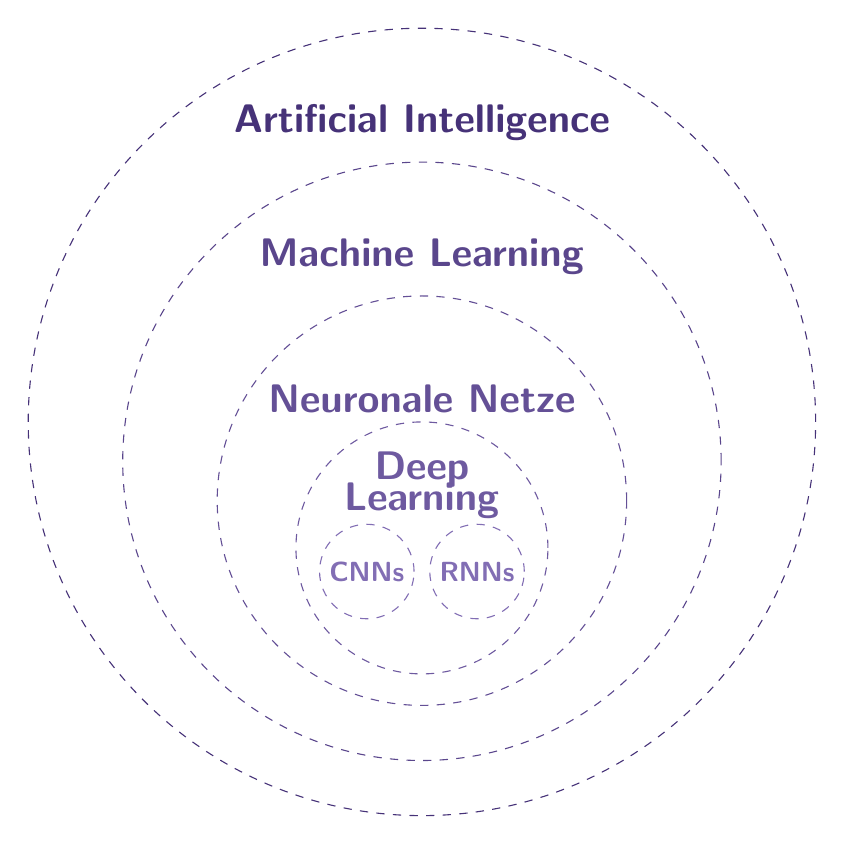
\begin{tikzpicture}[font=\sffamily]
		% Define colors
		\definecolor{outercolor}{RGB}{70,50,120}
		\definecolor{middlecolor}{RGB}{90,70,140}
		\definecolor{innermiddlecolor}{RGB}{100,80,150}
		\definecolor{innercolor}{RGB}{110,90,160}
		\definecolor{innermostcolor}{RGB}{130,110,180}
		% Outer circle (Artificial Intelligence)
		\draw[dashed, outercolor] (0,0) circle (5cm);
		\node[outercolor] at (0,3.8) {\Large\textbf{Artificial Intelligence}};
		% Middle circle (Machine Learning)
		\draw[dashed, middlecolor] (0,-0.5) circle (3.8cm);
		\node[middlecolor] at (0, 2.1) {\Large\textbf{Machine Learning}};
		% Inner-middle circle (Neuronale Netze)
		\draw[dashed, innermiddlecolor] (0,-1) circle (2.6cm);
		\node[innermiddlecolor] at (0,0.3) {\Large\textbf{Neuronale Netze}};
		% Inner circle (Deep Learning)
		\draw[dashed, innercolor] (0,-1.6) circle (1.6cm);
		\node[innercolor] at (0,-0.6) {\Large\textbf{Deep}};
		\node[innercolor] at (0,-1) {\Large\textbf{Learning}};
		% Innermost circles (CNNs and RNNs)
		\draw[dashed, innermostcolor] (-0.7,-1.9) circle (0.6cm);
		\node[innermostcolor] at (-0.7,-1.9) {\textbf{CNNs}};
		\draw[dashed, innermostcolor] (0.7,-1.9) circle (0.6cm);
		\node[innermostcolor] at (0.7,-1.9) {\textbf{RNNs}};
	\end{tikzpicture}
	\caption{Zusammenhang von Machine Learning, neuronalen Netzen, Deep Learning, \glspl{CNN} und \glspl{RNN}}
	\label{fig:ml-hierarchy}
\end{figure}

\subsection{Neuronale Netze}
\label{subsec:neuronale-netze}
Neuronale Netze sind eine Klasse von \gls{ML}-Modellen, die von der Funktionsweise des menschlichen Gehirns inspiriert sind \cite{RebalaGopinath2019AItM}. Sie bestehen aus miteinander verbundenen Neuronen, die in Schichten angeordnet sind:
\begin{itemize}
    \item Eingabeschicht (Input Layer): Nimmt die Eingabedaten auf
    \item Versteckte Schichten (Hidden Layer): Verarbeiten die Informationen
    \item Ausgabeschicht (Output Layer): Liefert das Ergebnis
\end{itemize}

Die Verbindungen zwischen den Neuronen haben Gewichte, die während des Trainings angepasst werden. Durch nichtlineare Aktivierungsfunktionen können neuronale Netze komplexe Zusammenhänge modellieren.

\subsubsection{Deep Learning}
\label{subsec:deep-learning}
Deep learning bezeichnet neuronale Netze die über viele versteckte Schichten verfügen \cite{RebalaGopinath2019AItM}, wodurch hierarchische Merkmale aus den Daten extrahiert werden können. Die Entwicklung von Deep Learning Algorithem führte in den letzten Jahren zu großen Fortschritten im Bereichen wie Bilderkennung, Sprachverarbeitung, Robotik oder auch \gls{OCR} \cite{jordan2015machine}.

Wichtige Konzepte im Deep Learning sind:
\begin{itemize}
	\item Backpropagation: Algorithmus zum effizienten Training durch Berechnung der Gradienten \cite{RebalaGopinath2019AItM}
	\item Regularisierung: Techniken zur Vermeidung von Overfitting \cite{jordan2015machine}
	\item Transfer Learning: Übertragung gelernter Merkmale auf neue Aufgaben \cite{jordan2015machine}
\end{itemize}


\subsubsection{Convolutional Neural Networks (CNNs)}
\label{subsubsec:cnn}
CNNs sind eine spezielle Art von neuronalen Netzen, die besonders für die Verarbeitung von Bilddaten geeignet sind \cite{RebalaGopinath2019AItM}. Sie nutzen Faltungsoperationen (Convolutions), um lokale Muster in den Eingabedaten zu erkennen. Im Kontext von \glspl{CNN} gibt es verschiedene gängige Ebenentypen \cite{RebalaGopinath2019AItM}:

\begin{itemize}
	\item Convolutional Layer: Anwendung von Filtern (Kernel) zur Merkmalserkennung
	\item ReLU (Rectified Linear Unit): nach einer Faltungsschicht wird häufig eine ReLU Funktion angewandt um die Komplexität des Modells zu reduzieren; dazu werden nichtlineare Merkmale eingeführt und negative Werte auf Null gesetzt
	\item Pooling Layer: Reduzierung der räumlichen Dimensionen
	\item Fully Connected Layer: verbinden jedes Neuron mit allen Neuronen der vorhergehenden Schicht; führen Klassifikation basierend auf extrahierten Merkmalen durch
\end{itemize}

CNNs haben sich als sehr leistungsfähig für Aufgaben wie Objekterkennung, Gesichtserkennung und autonomes Fahren erwiesen \cite{RebalaGopinath2019AItM}.

\section{Natural Language Processing (NLP)}
\label{sec:nlp}
\gls{NLP} befasst sich mit dem Verstehen und der Interpretation von menschlicher
Sprachen, gesprochen oder geschrieben, mit Hilfe maschineller Verarbeitung \cite{RebalaGopinath2019AItM}. \gls{NLP} ist nützlich für eine Vielzahl von
Anwendungen wie Spracherkennung, Sprachübersetzungen, Zusammenfassungen,
Fragebeantwortung, Spracherzeugung und Suchanwendungen.

\subsection{Tokenisierung}
\label{subsec:tokenisierung}
Die Tokenisierung ist ein fundamentaler Schritt in der Verarbeitung natürlicher Sprache. Hierbei wird ein Text in einzelne Einheiten, sogenannte Token, zerlegt \cite{RebalaGopinath2019AItM}. In den meisten Fällen entsprechen diese Token einzelnen Wörtern, können aber auch Satzzeichen oder andere bedeutungstragende Elemente umfassen \cite{RebalaGopinath2019AItM}. Ein einfacher Ansatz in Englischen Texten ist dazu beispielsweise den Text bei Leerzeichen zu trennen.

\subsection{Part-of-Speech Tagging}
\label{subsec:pos-tagging}
Im \gls{POS}-Tagging-Schritt wird jedes Wort in einem Text einer grammatikalischen Katgorie wie zum Beispiel Nomen, Verb, Adjektiv et cetera zugeordnet \cite{RebalaGopinath2019AItM}. Dieser Schritt ist wichtig, da die grammatikalische Funktion einens Wortes oft entscheidend für seine Bedeutung im Kontext ist.

\subsection{Named Entity Recognition}
\label{subsec:ner}
\gls{NER} ist eine zentrale Aufgabe im \gls{NLP}, bei der es darum geht, benannte Entitäten in einem Text zu identifizieren und zu klassifizieren \cite{nadeau2007survey}. Benannte Entitäten sind typischerweise Eigennamen von Personen, Organisationen, Orten, aber auch Zeitangaben, Währungen und andere spezifische Bezeichnungen.

\gls{NER}-Systeme müssen in der Lage sein, mehrdeutige Begriffe korrekt zu interpretieren. Beispielsweise kann "Tesla" je nach Kontext als Personenname, Unternehmensname oder als Einheit für magnetische Flussdichte verstanden werden \cite{RebalaGopinath2019AItM}.

Frühe \gls{NER}-Systeme basierten hauptsächlich auf manuell erstellten Regeln und Wörterbüchern \cite{nadeau2007survey}. Moderne Ansätze nutzen jedoch zunehmend maschinelle Lernverfahren, insbesondere überwachtes Lernen. Dabei werden Modelle auf großen, annotierten Texten trainiert, um Muster und Kontexte zu erkennen, die auf benannte Entitäten hindeuten \cite{nadeau2007survey}.
Diese beiden Ansätze können auch kombiniert werden, um die Flexibilität des maschinellen Lernens mit domänenspezifischen Wissen zu kombinieren \cite{nadeau2007survey}. Dies verbessert die Genauigkeit und hat sich als besonders effektiv erwiesen. Die Leistungsfähigkeit wird dabei typischerweise anhand von Präzision und Recall gemessen.

\section{Transformer-Architekturen und Large Language Models}
\label{sec:transformers-llms}

\subsection{Transformer-Architektur}
\label{subsec:transformer-architecture}

Die Transformer-Architektur, erstmals von \textcite{VaswaniAshish2023AIAY}. vorgestellt, revolutionierte das Feld des maschinellen Lernens für natürliche Sprache. Im Gegensatz zu früheren rekurrenten oder faltungsbasierten Modellen basiert der Transformer vollständig auf Aufmerksamkeitsmechanismen (Attention), was eine effizientere Verarbeitung langer Sequenzen ermöglicht.

Kernelemente der Transformer-Architektur sind \cite{VaswaniAshish2023AIAY}:
\begin{itemize}
	\item Multi-Head Attention: Ermöglicht dem Modell, verschiedene Aspekte der Eingabe parallel zu berücksichtigen.
	\item Positionscodierung: Fügt Informationen über die Reihenfolge der Tokens hinzu, da die Attention-Mechanismen selbst keine Reihenfolge berücksichtigen.
	\item Feed-Forward-Netzwerke: Verarbeiten die Ausgaben der Attention-Layer weiter.
	\item Residuale Verbindungen und Layer-Normalisierung: Verbessern den Informationsfluss und stabilisieren das Training.
\end{itemize}

Die Transformer-Architektur hat sich aufgrund ihrer Skalierbarkeit und Effizienz als Grundlage für viele moderne Sprachmodelle etabliert \cite{VaswaniAshish2023AIAY}.

\subsection{BERT und verwandte Modelle}
\label{subsec:bert}

Die von \textcite{DevlinJacob2019BPoD} vorgestellte \gls{BERT}-Technologie war ein weiterer bedeutender Fortschritt in der Anwendung von Transformer-Architekturen. BERT verwendet eine bidirektionale Vortrainingsmethode, die es dem Modell ermöglicht, Kontext aus beiden Richtungen zu berücksichtigen \cite{DevlinJacob2019BPoD}.

Wichtige Aspekte dieses Trainingsprozesses sind \cite{DevlinJacob2019BPoD}:
\begin{itemize}
	\item Masked Language Model (MLM): Trainiert das Modell, maskierte Wörter in einem Satz vorherzusagen.
	\item Next Sentence Prediction (NSP): Trainiert das Modell, die Beziehung zwischen Satzpaaren zu verstehen.
\end{itemize}
 \gls{BERT}\cite{DevlinJacob2019BPoD} sowie Varianten wie ALBERT\cite{LanZhenzhong2019AALB} oder RoBERTa\cite{liu2019robertarobustlyoptimizedbert} haben zu signifikanten Verbesserungen in vielen natürlichen Sprachverarbeitungsaufgaben geführt.

\subsection{Large Language Models (LLMs)}
\label{subsec:llms}
Large Language Models (LLMs) stellen eine bedeutende Weiterentwicklung in der Verarbeitung natürlicher Sprache dar. Diese Transformer-basierten Modelle zeichnen sich durch eine enorme Anzahl von Parametern aus und werden auf sehr großen Textkorpora trainiert \cite{VaswaniAshish2023AIAY}.

Bemerkenswerte Fähigkeiten von \glspl{LLM} sind dabei:

\begin{itemize}[]
	\item Skalierung: Die Leistung verbessert sich oft mit zunehmender Modellgröße und Datenmenge \cite{TouvronHugo2023LOaE}.
	 
	\item Emergente Fähigkeiten: Unerwartete Fähigkeiten, die erst ab einer bestimmten Modellgröße auftreten, wie beispielsweise das Erkennen von Musten in daten, verbessertes Kontext Verständnis, komplexes Argumentieren und kreatives Schreiben \cite{BrownTomB2020LMaF}.
	 
	\item Few-Shot Learning: Die Fähigkeit, neue Aufgaben mit wenigen oder keinen spezifischen Trainingsbeispielen zu lernen \cite{BrownTomB2020LMaF}.
	
	\item Transfer Learning: LLMs können das auf großen allgemeinen Textkorpora erlernte Wissen auf spezifische Aufgaben übertragen \cite{DevlinJacob2019BPoD}.
	
	\item Multimodalität: Neuere LLMs integrieren zunehmend Fähigkeiten zur Verarbeitung verschiedener Modalitäten wie Text und Bilder \cite{LiJunnan2023BBLP}.
\end{itemize}

\subsubsection{LLaMA}
\label{subsubsec:LLaMA}
Für die Aufgabenstellung besonders interessant sind, die von \textcite{TouvronHugo2023LOaE} erstmals vorgestellten Modelle der LLaMa Reihe. Diese sind in Größen von 7-65 Milliarden Parametern verfügbar und wurden auf Basis von öffentlichen Daten trainiert \cite{TouvronHugo2023LOaE}. Dabei wurde gezeigt, dass es möglich ist, leistungsfähige Sprachmodelle mit öffentlichen Daten zu trainieren, was die Forschung und Entwicklung in diesem Bereich demokratisiert. Die Autoren betonen, dass LLaMA auf einer Vielzahl von Benchmarks, einschließlich Aufgaben zum Schlussfolgern, Lesen und mathematischem Denken, wettbewerbsfähige oder überlegene Ergebnisse im Vergleich zu Modellen ähnlicher Größe erzielt \cite{TouvronHugo2023LOaE}.
Die neueste Version, LLaMa 3, erweitert diese Fähigkeiten deutlich. Sie bietet Modelle mit bis zu 405 Milliarden Parametern, die auf etwa 15 Billionen mehrsprachigen Tokens trainiert wurden \cite{HartshornAnthony2024TL3H}. Besonders die Mehrsprachigkeit sowie die deutlich verbesserte Leistung, die laut den Autoren mit führenden Modellen wie GPT-4 vergleichbar ist, kombiniert mit der Tatsache, dass LLAMA 3, einschließlich des 405B-Modells, von Meta öffentlich freigegebn wurde, machen das System zur Umsetzung von Techniken, wie \gls{LMDX}\ref{subsec:language-model-basierte-document-information-extraction} besonders interressant.

\subsection{Herausforderungen und Einschränkungen}
\label{subsec:llm-challenges}

Trotz ihrer beeindruckenden Fähigkeiten stehen \glspl{LLM} vor mehreren Herausforderungen:

\begin{itemize}
	\item Rechenaufwand und Energieverbrauch: Das Training großer Modelle erfordert erhebliche Rechenressourcen. \textcite{TouvronHugo2023LOaE} berichten, dass das Training ihrer größten LLAMA-Modelle mehrere Tage auf Tausenden von GPUs benötigte.
	
	\item Bias und Fairness: \glspl{LLM} können voreingenommene oder unfaire Ausgaben produzieren, die gesellschaftliche Vorurteile widerspiegeln. \textcite{BrownTomB2020LMaF} diskutieren dieses Problem und betonen die Notwendigkeit, es bei der Entwicklung und Anwendung von \glspl{LLM} zu berücksichtigen.
	
	\item Halluzinationen: \glspl{LLM} können plausibel klingende, aber falsche Informationen generieren. \textcite{JiangZhengbao2020HCWK} untersuchen dieses Phänomen und betonen die Schwierigkeit, den wahren Wissensstand eines \gls{LLM} zu bestimmen.
	
	\item Interpretierbarkeit: Es ist oft schwierig zu verstehen, wie \glspl{LLM} zu bestimmten Ausgaben gelangen. \textcite{DevlinJacob2019BPoD} erwähnen diese Herausforderung im Kontext von BERT, was auch für größere \glspl{LLM} relevant bleibt.
	
	\item Datenschutz und ethische Bedenken: Die Verwendung großer Mengen an Trainingsdaten wirft Fragen zum Datenschutz und zur ethischen Nutzung von Informationen auf \cite{TouvronHugo2023LOaE}.
\end{itemize}

\section{Evaluation und Metriken}
\label{sec:evaluation-metrics}

\subsection{Precision, Recall und F1-Score}
\label{subsec:precision-recall-f1}

\subsection{Micro-F1 und Macro-F1}
\label{subsec:micro-macro-f1}

\section{Lernparadigmen und Aufgabenkategorien}
\label{sec:lernparadigmen-aufgabenkategorien}

\subsection{Transfer Learning}
\label{subsec:transfer-learning}

\subsection{Few-Shot Learning}
\label{subsec:few-shot-learning}

\subsection{Zero-Shot Learning}
\label{subsec:zero-shot-learning}

\subsection{Meta-Learning}
\label{subsec:meta-learning}

\subsection{Multitask Learning}
\label{subsec:multitask-learning}